\documentclass{extbook}[14pt]
\usepackage{multicol, enumerate, enumitem, hyperref, color, soul, setspace, parskip, fancyhdr, amssymb, amsthm, amsmath, bbm, latexsym, units, mathtools}
\everymath{\displaystyle}
\usepackage[headsep=0.5cm,headheight=0cm, left=1 in,right= 1 in,top= 1 in,bottom= 1 in]{geometry}
\usepackage{dashrule}  % Package to use the command below to create lines between items
\newcommand{\litem}[1]{\item #1

\rule{\textwidth}{0.4pt}}
\pagestyle{fancy}
\lhead{}
\chead{Answer Key for Makeup Progress Quiz 3 Version C}
\rhead{}
\lfoot{4315-3397}
\cfoot{}
\rfoot{Fall 2020}
\begin{document}
\textbf{This key should allow you to understand why you choose the option you did (beyond just getting a question right or wrong). \href{https://xronos.clas.ufl.edu/mac1105spring2020/courseDescriptionAndMisc/Exams/LearningFromResults}{More instructions on how to use this key can be found here}.}

\textbf{If you have a suggestion to make the keys better, \href{https://forms.gle/CZkbZmPbC9XALEE88}{please fill out the short survey here}.}

\textit{Note: This key is auto-generated and may contain issues and/or errors. The keys are reviewed after each exam to ensure grading is done accurately. If there are issues (like duplicate options), they are noted in the offline gradebook. The keys are a work-in-progress to give students as many resources to improve as possible.}

\rule{\textwidth}{0.4pt}

\begin{enumerate}\litem{
Solve the rational equation below. Then, choose the interval(s) that the solution(s) belongs to.
\[ \frac{3}{-7x + 9} + -2 = \frac{9}{-42x + 54} \]

The solution is \( x = 1.179 \), which is option B.\begin{enumerate}[label=\Alph*.]
\item \( \text{All solutions lead to invalid or complex values in the equation.} \)

This corresponds to thinking $x = 1.179$ leads to dividing by zero in the original equation, which it does not.
\item \( x \in [0.18,2.18] \)

* $x = 1.179$, which is the correct option.
\item \( x_1 \in [0.2, 1.6] \text{ and } x_2 \in [1.45,2.01] \)

$x = 1.179 \text{ and } x = 1.714$, which corresponds to getting the correct solution and believing there should be a second solution to the equation.
\item \( x \in [-2.1,-0.2] \)

$x = -1.393$, which corresponds to not distributing the factor $-7x + 9$ correctly when trying to eliminate the fraction.
\item \( x_1 \in [-2.1, -0.2] \text{ and } x_2 \in [1.09,1.32] \)

$x = -1.393 \text{ and } x = 1.179$, which corresponds to getting the correct solution and believing there should be a second solution to the equation.
\end{enumerate}

\textbf{General Comment:} Distractors are different based on the number of solutions. Remember that after solving, we need to make sure our solution does not make the original equation divide by zero!
}
\litem{
Solve the rational equation below. Then, choose the interval(s) that the solution(s) belongs to.
\[ \frac{-2x}{-5x + 5} + \frac{-3x^{2}}{20x^{2} -20} = \frac{5}{-4x -4} \]

The solution is \( \text{There are two solutions: } x = 0.686 \text{ and } x = -7.286 \), which is option E.\begin{enumerate}[label=\Alph*.]
\item \( x_1 \in [-0.31, 5.69] \text{ and } x_2 \in [-3,4] \)


\item \( \text{All solutions lead to invalid or complex values in the equation.} \)


\item \( x \in [-6,0] \)


\item \( x \in [-7.29,-3.29] \)


\item \( x_1 \in [-0.31, 5.69] \text{ and } x_2 \in [-10.29,-4.29] \)

* $x = 0.686 \text{ and } x = -7.286$, which is the correct option.
\end{enumerate}

\textbf{General Comment:} Distractors are different based on the number of solutions. Remember that after solving, we need to make sure our solution does not make the original equation divide by zero!
}
\litem{
Choose the graph of the equation below.
\[ f(x) = \frac{1}{(x - 3)^2} - 2 \]

The solution is the graph below, which is option B.
\begin{center}
    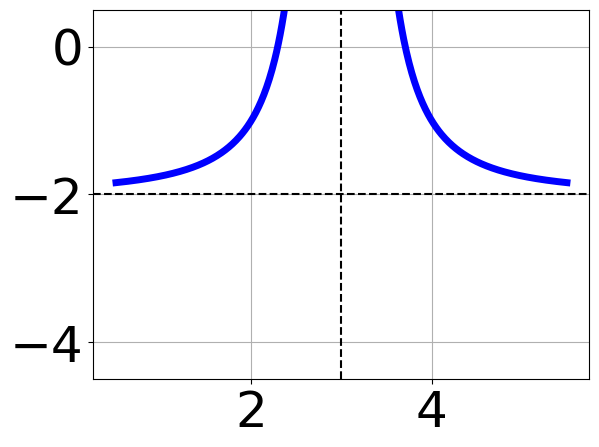
\includegraphics[width=0.3\textwidth]{../Figures/rationalEquationToGraphCopyBC.png}
\end{center}\begin{enumerate}[label=\Alph*.]
\begin{multicols}{2}
\item 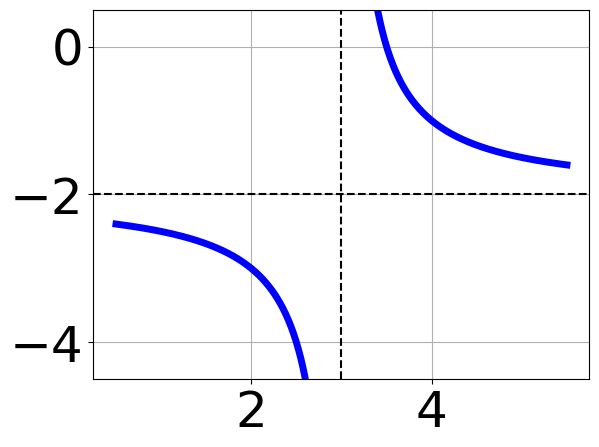
\includegraphics[width = 0.3\textwidth]{../Figures/rationalEquationToGraphCopyAC.png}
\item 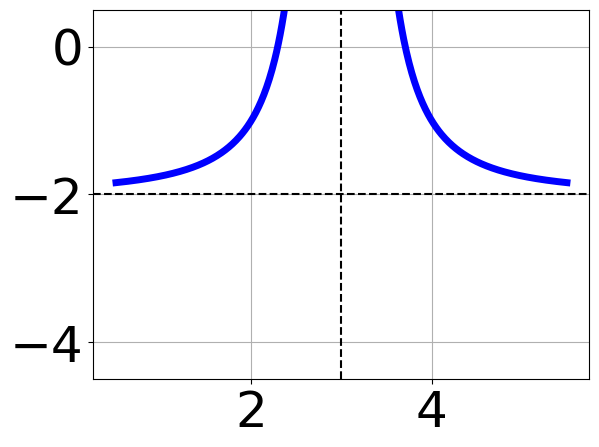
\includegraphics[width = 0.3\textwidth]{../Figures/rationalEquationToGraphCopyBC.png}
\item 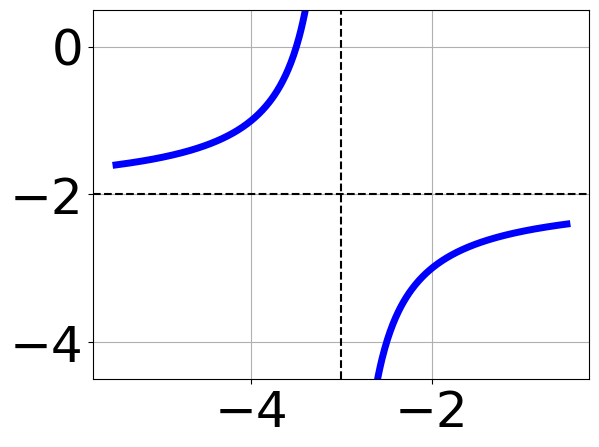
\includegraphics[width = 0.3\textwidth]{../Figures/rationalEquationToGraphCopyCC.png}
\item 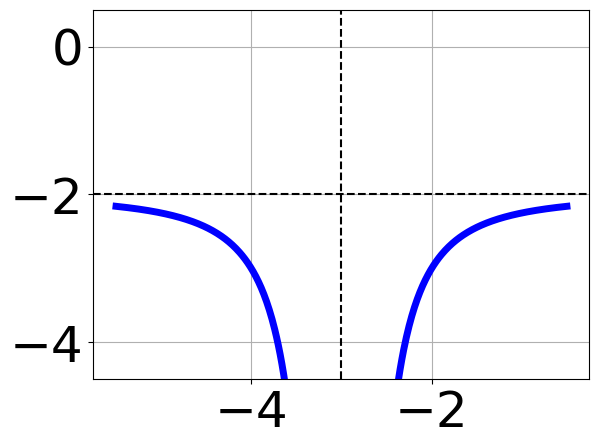
\includegraphics[width = 0.3\textwidth]{../Figures/rationalEquationToGraphCopyDC.png}
\end{multicols}\item None of the above.\end{enumerate}
\textbf{General Comment:} Remember that the general form of a basic rational equation is $ f(x) = \frac{a}{(x-h)^n} + k$, where $a$ is the leading coefficient (and in this case, we assume is either $1$ or $-1$), $n$ is the degree (in this case, either $1$ or $2$), and $(h, k)$ is the intersection of the asymptotes.
}
\litem{
Determine the domain of the function below.
\[ f(x) = \frac{3}{15x^{2} +43 x + 30} \]

The solution is \( \text{All Real numbers except } x = -1.667 \text{ and } x = -1.200. \), which is option C.\begin{enumerate}[label=\Alph*.]
\item \( \text{All Real numbers except } x = a, \text{ where } a \in [-30.13, -29.84] \)

All Real numbers except $x = -30.000$, which corresponds to removing a distractor value from the denominator.
\item \( \text{All Real numbers.} \)

This corresponds to thinking the denominator has complex roots or that rational functions have a domain of all Real numbers.
\item \( \text{All Real numbers except } x = a \text{ and } x = b, \text{ where } a \in [-1.67, -1.48] \text{ and } b \in [-1.3, -1.2] \)

All Real numbers except $x = -1.667$ and $x = -1.200$, which is the correct option.
\item \( \text{All Real numbers except } x = a, \text{ where } a \in [-1.67, -1.48] \)

All Real numbers except $x = -1.667$, which corresponds to removing only 1 value from the denominator.
\item \( \text{All Real numbers except } x = a \text{ and } x = b, \text{ where } a \in [-30.13, -29.84] \text{ and } b \in [-15.09, -14.76] \)

All Real numbers except $x = -30.000$ and $x = -15.000$, which corresponds to not factoring the denominator correctly.
\end{enumerate}

\textbf{General Comment:} Recall that dividing by zero is not a real number. Therefore the domain is all real numbers \textbf{except} those that make the denominator 0.
}
\litem{
Choose the equation of the function graphed below.

\begin{center}
    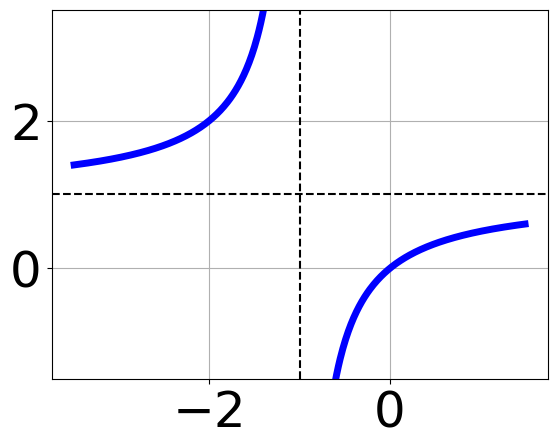
\includegraphics[width=0.5\textwidth]{../Figures/rationalGraphToEquationC.png}
\end{center}




The solution is \( f(x) = \frac{-1}{x + 1} + 1 \), which is option B.\begin{enumerate}[label=\Alph*.]
\item \( f(x) = \frac{-1}{(x + 1)^2} + 1 \)

Corresponds to thinking the graph was a shifted version of $\frac{1}{x^2}$.
\item \( f(x) = \frac{-1}{x + 1} + 1 \)

This is the correct option.
\item \( f(x) = \frac{1}{(x - 1)^2} + 1 \)

Corresponds to thinking the graph was a shifted version of $\frac{1}{x^2}$, using the general form $f(x) = \frac{a}{x+h}+k$, and the opposite leading coefficient.
\item \( f(x) = \frac{1}{x - 1} + 1 \)

Corresponds to using the general form $f(x) = \frac{a}{x+h}+k$ and the opposite leading coefficient.
\item \( \text{None of the above} \)

This corresponds to believing the vertex of the graph was not correct.
\end{enumerate}

\textbf{General Comment:} Remember that the general form of a basic rational equation is $ f(x) = \frac{a}{(x-h)^n} + k$, where $a$ is the leading coefficient (and in this case, we assume is either $1$ or $-1$), $n$ is the degree (in this case, either $1$ or $2$), and $(h, k)$ is the intersection of the asymptotes.
}
\litem{
Determine the domain of the function below.
\[ f(x) = \frac{6}{12x^{2} -25 x + 12} \]

The solution is \( \text{All Real numbers except } x = 0.750 \text{ and } x = 1.333. \), which is option C.\begin{enumerate}[label=\Alph*.]
\item \( \text{All Real numbers.} \)

This corresponds to thinking the denominator has complex roots or that rational functions have a domain of all Real numbers.
\item \( \text{All Real numbers except } x = a \text{ and } x = b, \text{ where } a \in [11.2, 12.4] \text{ and } b \in [11.2, 12.4] \)

All Real numbers except $x = 12.000$ and $x = 12.000$, which corresponds to not factoring the denominator correctly.
\item \( \text{All Real numbers except } x = a \text{ and } x = b, \text{ where } a \in [0.2, 1.2] \text{ and } b \in [0.9, 2.1] \)

All Real numbers except $x = 0.750$ and $x = 1.333$, which is the correct option.
\item \( \text{All Real numbers except } x = a, \text{ where } a \in [11.2, 12.4] \)

All Real numbers except $x = 12.000$, which corresponds to removing a distractor value from the denominator.
\item \( \text{All Real numbers except } x = a, \text{ where } a \in [0.2, 1.2] \)

All Real numbers except $x = 0.750$, which corresponds to removing only 1 value from the denominator.
\end{enumerate}

\textbf{General Comment:} Recall that dividing by zero is not a real number. Therefore the domain is all real numbers \textbf{except} those that make the denominator 0.
}
\litem{
Solve the rational equation below. Then, choose the interval(s) that the solution(s) belongs to.
\[ \frac{3x}{-3x + 3} + \frac{-7x^{2}}{-9x^{2} +30 x -21} = \frac{-4}{3x -7} \]

The solution is \( \text{There are two solutions: } x = 0.372 \text{ and } x = 16.128 \), which is option C.\begin{enumerate}[label=\Alph*.]
\item \( x \in [1.68,2.41] \)


\item \( x \in [15.89,16.77] \)


\item \( x_1 \in [-2.06, 1.97] \text{ and } x_2 \in [10.13,24.13] \)

* $x = 0.372 \text{ and } x = 16.128$, which is the correct option.
\item \( x_1 \in [-2.06, 1.97] \text{ and } x_2 \in [-3,7] \)


\item \( \text{All solutions lead to invalid or complex values in the equation.} \)


\end{enumerate}

\textbf{General Comment:} Distractors are different based on the number of solutions. Remember that after solving, we need to make sure our solution does not make the original equation divide by zero!
}
\litem{
Solve the rational equation below. Then, choose the interval(s) that the solution(s) belongs to.
\[ \frac{-9}{-8x -7} + 8 = \frac{-9}{-64x -56} \]

The solution is \( x = -0.998 \), which is option A.\begin{enumerate}[label=\Alph*.]
\item \( x \in [-2.0,1.0] \)

* $x = -0.998$, which is the correct option.
\item \( x_1 \in [-1, 0] \text{ and } x_2 \in [-2.1,0.3] \)

$x = -0.998 \text{ and } x = -0.875$, which corresponds to getting the correct solution and believing there should be a second solution to the equation.
\item \( \text{All solutions lead to invalid or complex values in the equation.} \)

This corresponds to thinking $x = -0.998$ leads to dividing by zero in the original equation, which it does not.
\item \( x \in [0.75,3.75] \)

$x = 0.752$, which corresponds to not distributing the factor $-8x -7$ correctly when trying to eliminate the fraction.
\item \( x_1 \in [-1, 0] \text{ and } x_2 \in [0.2,0.9] \)

$x = -0.998 \text{ and } x = 0.752$, which corresponds to getting the correct solution and believing there should be a second solution to the equation.
\end{enumerate}

\textbf{General Comment:} Distractors are different based on the number of solutions. Remember that after solving, we need to make sure our solution does not make the original equation divide by zero!
}
\litem{
Choose the equation of the function graphed below.

\begin{center}
    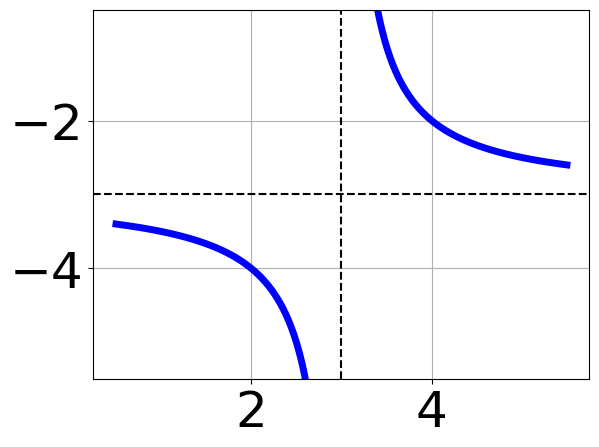
\includegraphics[width=0.5\textwidth]{../Figures/rationalGraphToEquationCopyC.png}
\end{center}




The solution is \( \text{None of the above as it should be } f(x) = \frac{1}{x - 3} - 3 \), which is option E.\begin{enumerate}[label=\Alph*.]
\item \( f(x) = \frac{-1}{x - 3} - 3 \)

Corresponds to using the general form $f(x) = \frac{a}{x-h}+k$ and the opposite leading coefficient.
\item \( f(x) = \frac{1}{(x + 3)^2} - 3 \)

Corresponds to thinking the graph was a shifted version of $\frac{1}{x^2}$.
\item \( f(x) = \frac{-1}{(x - 3)^2} - 3 \)

Corresponds to thinking the graph was a shifted version of $\frac{1}{x^2}$, using the general form $f(x) = \frac{a}{x-h}+k$, and the opposite leading coefficient.
\item \( f(x) = \frac{1}{x + 3} - 3 \)

The $x$-value of the equation does not match the graph.
\item \( \text{None of the above} \)

None of the equation options were the correct equation.
\end{enumerate}

\textbf{General Comment:} Remember that the general form of a basic rational equation is $ f(x) = \frac{a}{(x-h)^n} + k$, where $a$ is the leading coefficient (and in this case, we assume is either $1$ or $-1$), $n$ is the degree (in this case, either $1$ or $2$), and $(h, k)$ is the intersection of the asymptotes.
}
\litem{
Choose the graph of the equation below.
\[ f(x) = \frac{1}{x + 2} + 3 \]

The solution is the graph below, which is option B.
\begin{center}
    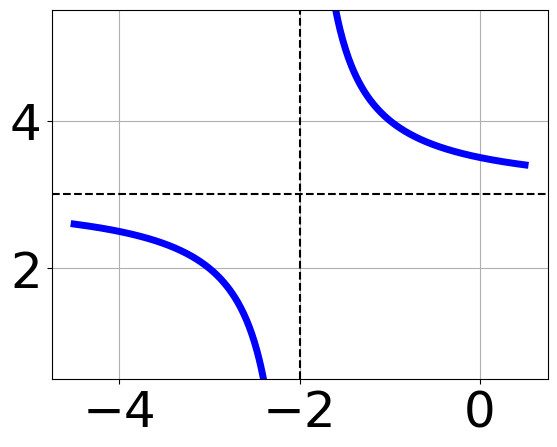
\includegraphics[width=0.3\textwidth]{../Figures/rationalEquationToGraphBC.png}
\end{center}\begin{enumerate}[label=\Alph*.]
\begin{multicols}{2}
\item 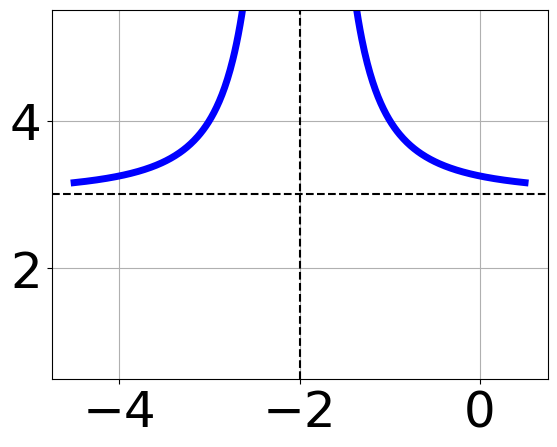
\includegraphics[width = 0.3\textwidth]{../Figures/rationalEquationToGraphAC.png}
\item 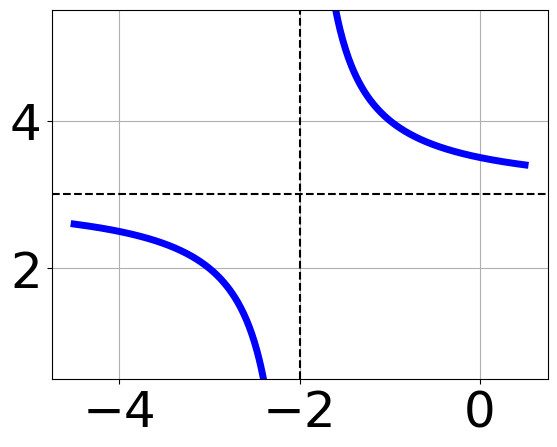
\includegraphics[width = 0.3\textwidth]{../Figures/rationalEquationToGraphBC.png}
\item 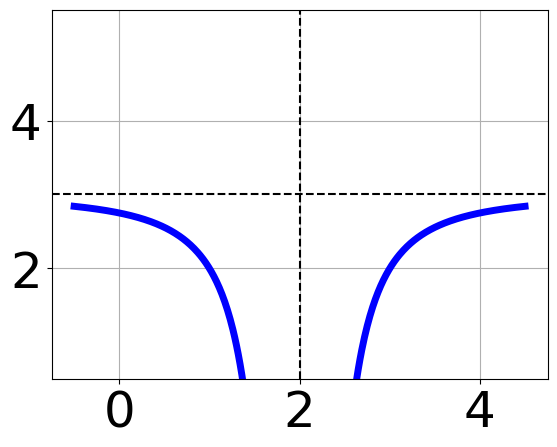
\includegraphics[width = 0.3\textwidth]{../Figures/rationalEquationToGraphCC.png}
\item 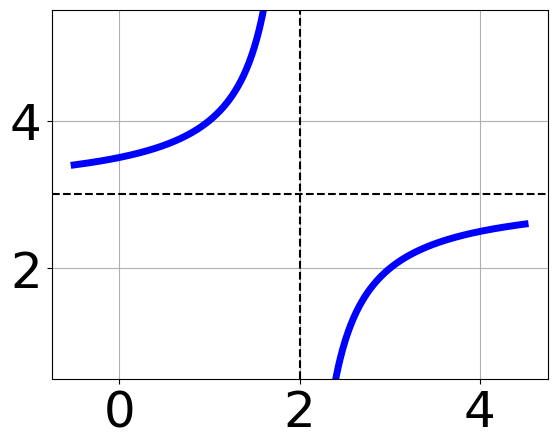
\includegraphics[width = 0.3\textwidth]{../Figures/rationalEquationToGraphDC.png}
\end{multicols}\item None of the above.\end{enumerate}
\textbf{General Comment:} Remember that the general form of a basic rational equation is $ f(x) = \frac{a}{(x-h)^n} + k$, where $a$ is the leading coefficient (and in this case, we assume is either $1$ or $-1$), $n$ is the degree (in this case, either $1$ or $2$), and $(h, k)$ is the intersection of the asymptotes.
}
\end{enumerate}

\end{document}